\documentclass{standalone}
\usepackage{tikz}
\usetikzlibrary{arrows.meta}
\tikzset{label/.style = {inner sep=1pt, fill=white}}
%\tikzset{nd/.style={circle, inner sep=0pt}}
\tikzset{nd/.style={inner sep=1pt}}
\tikzset{>=Latex}
\tikzset{arc/.style = {->, semithick, >=Latex}}
\begin{document}
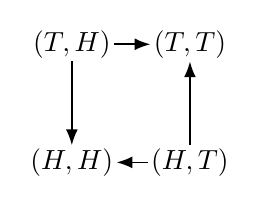
\begin{tikzpicture}
    \node[nd] (A) at (0,0) {$(H,H)$};
    \node[nd] (B) at (0,1.5) {$(T,H)$};
    \node[nd] (C) at (1.5,0) {$(H,T)$};
    \node[nd] (D) at (1.5,1.5) {$(T,T)$};
    \draw[arc] (B) to (A);
    \draw[arc] (C) to (A);
    \draw[arc] (B) to (D);
    \draw[arc] (C) to (D);
\end{tikzpicture}
\end{document}